\begin{frame}{Circuits and protocols}

    \begin{theorem}
        There is a {\color{blue}monotone} boolean circuit for function $f$ of size $S$ iff there is a
        boolean communication game of size $S$ for a relation $\Bit$ {\color{blue}$(\MBit)$} $(U =
        f^{-1}(1), V = f^{-1}(0))$.
    \end{theorem}
    
    \pause
    Proof ($\Leftarrow$):
    \begin{columns}[t]
		\begin{column}{0.65\textwidth}
            \vspace{-5mm}
            \begin{enumerate}
                \item<3-> $(H, A, B)$ is a game, $R_h = U_h \times V_h$ is a rectangle for $h \in H$.
                \item<4-> By induction we create circuits for $f_h$ such that $f_h(U_h) = 1$ and
                    $f_h(V_h) = 0$.
                \item<5-> If a leaf $h$ is marked by $i$ then $f_h = x_i$ or $f_h = \neg x_i$.
                \item<6-> For an inner vertex $h$ with children $h', h''$: $f_h = f_{h'} \land f_{h''}$
                    or $f_h = f_{h'} \lor f_{h''}$.
            \end{enumerate}
        \end{column}
        
		\begin{column}{0.35\textwidth}
            \only<5>{For all $u \in U_h$ and $v \in V_h$, $u_i \neq v_i$ $\Rightarrow$ if $u_i = 1$ and
            	$v_i = 0$ then $f_h = x_i$ else $f_h = \neg x_i$.
            }
            \only<6->{
                \vspace{-6mm}
                \begin{center}
                	\tikzstyle{end} = [thin, circle, minimum size = 0.1cm, draw, inner sep = 0.1pt]
\tikzstyle{leaf} = [thin, circle, minimum size = 0.6cm, draw, inner sep = 0.1pt, blue]
\tikzstyle{inner} = [thin, circle, minimum size = 0.2cm, draw, inner sep = 0.1pt, black]
            


\tikzstyle{ed} = [thick, ->, draw, black]

    
\begin{tikzpicture}[black]
    \draw[very thick] (0, 0) rectangle (3, 3);
	\draw[fill = gray!80!white] (0.8, 0.8) rectangle (2.1, 2.2) node[below left] {\scriptsize $R_h$};
    \only<6>{
        \draw[fill = green!20!white, opacity = 0.5, rounded corners] (0.4, 0.4) rectangle (1.4, 2.9) node[below left]
	    {\scriptsize $R_{h'}$};
	    \draw[fill = red!10!white, opacity = 0.5, rounded corners] (1.1, 0.6) rectangle (2.8, 2.5) node[below left]
	    {\scriptsize $R_{h''}$};
    }
    \only<7>{
        \draw[fill = green!20!white, opacity = 0.5, rounded corners] (0.4, 1.2) rectangle (2.8, 2.7) node[below left]
	    {\scriptsize $R_{h'}$};
	    \draw[fill = red!10!white, opacity = 0.5, rounded corners] (0.6, 1.4) rectangle (2.75, 0.5) node[above left]
	    {\scriptsize $R_{h''}$};
    }
\end{tikzpicture}
                    
	                \only<6>{
                        $f_{h'}(U_h) = f_{h''}(U_h) = 1$

                        $f_{h} = f_{h'} \land f_{h''}$
                    }
                    \only<7>{
                        $f_{h'}(V_h) = f_{h''}(V_h) = 0$

                        $f_{h} = f_{h'} \lor f_{h''}$
                    }
                \end{center}
            }
		\end{column}
	\end{columns}
\end{frame}

\begin{frame}{From $\CP$ to games}

    \begin{lemma}
        \begin{itemize}
            \item $\varphi(x, y)$ is unsatisfiable CNF formula;
            \item $U$ is set of assignments to $x$, $V$ is a set of assignments to $y$;
            \item there is a $\CP$ proof of $\varphi$ of size $S$
        \end{itemize}
        $\Rightarrow$ there is a real communication game for sets $(U, V)$ and a canonical search problem $\Search_{\varphi}$
        of size $S$. 
    \end{lemma}

    \pause
    Proof:
    \pause
    \begin{itemize}
        \item $H$ is a graph of the proof of $\phi$ with inverted edges;
        \pause
        \item $h \in H$, this vertex corresponds to inequalities $f(x) + \ell(y) \ge c$;
        \pause
        \item $A(h, u) = -f(u)$ and $B(h, v) = \ell(v) - c$;
        \pause    
        \item $A(h, u) > B(h, v)$ iff $f(u) + \ell(v) < c$;
        \pause
        \item root corresponds to $1 \ge 0$ $\Rightarrow$ root is valid for all inputs;
        \pause
        \item if all children of $h$ is not valid then $h$ is not valid.
    \end{itemize}
\end{frame}
